\documentclass[10pt,twocolumn]{article}
% Packages
\usepackage{times}
\usepackage[fleqn]{amsmath}
\usepackage{amssymb}
\usepackage{anysize}
\usepackage{multicol}
\usepackage{graphicx}
\usepackage{booktabs}
\usepackage{titlesec}
\usepackage{float}
\usepackage{natbib}
\usepackage[english]{babel}
\usepackage[autolanguage]{numprint}
%\restylefloat{table}
\usepackage[tableposition=top]{caption}
% Macros
\newcommand{\np}{\numprint}
% Options
\marginsize{2.5cm}{1.5cm}{1cm}{1cm}
\setlength{\columnsep}{18.0pt}
% Title spec
\title{COMP3130 -- Group Project in Computer Science\\ Warm-up Project -- 4$\times$4$\times$4 TicTacToe Agent}
\date{March 24, 2012}
\author{Andrew Haigh -- u4667010;\\ Timothy Cosgrove -- u4843619;\\ Joshua Nelson -- u4850020}
% Section styling
\titleformat{\section}%
  {\large\itshape}%
  {\thesection.}{.5em}{}%
  [\vspace{1ex}\titlerule]%
\titleformat{\subsection}%
  {\itshape}%
  {\thesubsection.}{.5em}{}%
\begin{document}
\onecolumn
\maketitle
\twocolumn
\section{Abstract}
The purpose of this project was to implement an intelligent agent to play 3
dimensional 4 by 4 by 4 Tic Tac Toe. We chose to implement this in C, with a
pipe interface to python. This allowed us to use python's 3D libraries for visualisation
while utilising the speed of a compiled C program.

\section{Solution Overview}
The core of the agent is implemented with a combination of minimax and $\alpha$-$\beta$ pruning.

Board states are stored simply as a 3 dimensional array of chars; but this data is passed
through the program as a struct including extra information such as a heuristic evaluation
of the state, a move number indicating how many positions have been filled,
and a short list of the array coordinates that are occupied (for fast iteration over the array).
Once the minimax program reaches a fixed cut-off depth we select a state based on
this heuristic. For testing purposes all code is compiled with the -g flag. This allows
us to use the program \texttt{gprof} to analyse running time and total number of function calls
(this is used to optimise and evaluate the effectiveness of $\alpha$-$\beta$ pruning).

\subsection{Overview of modules}
\texttt{visualisation.py:}
\begin{itemize}
\item The python module which takes user input (to play against the computer) and displays the game board using VPython
\item This is the main program, it creates a sub-process (\texttt{worker.c}) which returns
board states to display
\item Contains several visualisation options such as labels on each square and even
red-cyan stereoscopic 3D. See \texttt{README} for details.
\end{itemize}
\begin{figure}[h]
  \begin{center}
    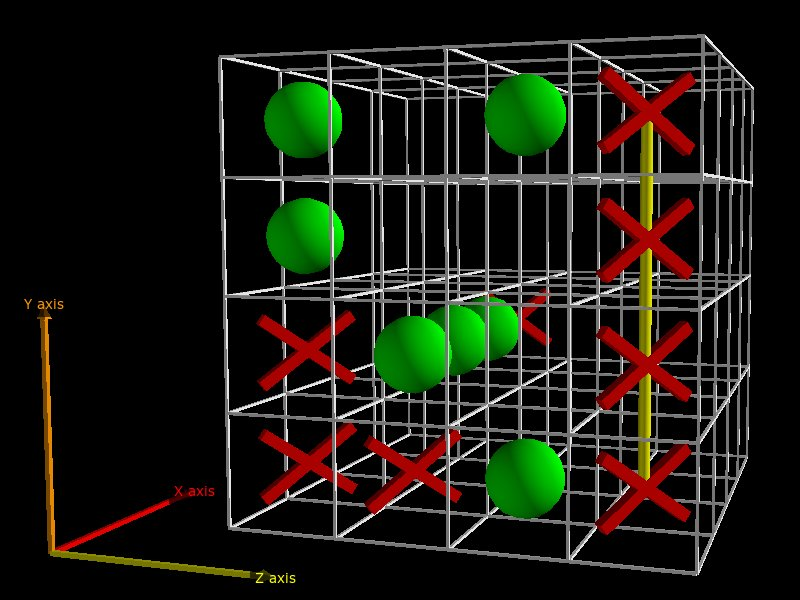
\includegraphics[width=2.5in]{vis.jpg}
  \end{center}
  \caption{Example of a game visualisation}
  \label{fig:vis}
\end{figure}
\texttt{worker.c:}
\begin{itemize}
\item The link module which handles communication between python and C
\item Calls code from \texttt{state\_functions.c} to start minimax and pick the next move
\end{itemize}
\texttt{state\_functions.c:}
\begin{itemize}
\item Contains all core functionality of the AI agent including minimax functions and state
evaluation functions
\item Includes a simple victory function which checks if a player has won with a line nearby to
the most recent move. (comprehensive victory checks are made in \texttt{visualisation.py})
\end{itemize}

\section{State Space for 4$\times$4$\times$4}
In the original scope of this project we had intended to examine the entire state space
before making a move. However, the state space is in fact exceedingly large. Considering all
possible states we have $3^{64}$, but many of these (far more than half) are illegal or unreachable.
According to \cite{Patashnik1980}, after 18 moves (under perfect play by player 1)
the game will be over or in a state where every move is forced. With this in mind we can 
consider a more reasonable upper bound on the states we must examine:
 \[\binom{64}{18} = 3601688791018080\]
If we assume we can examine 1 state per clock cycle (a completely and utterly unreasonable assumption) it would
still take over 250 hours to search this reduced state space on a 4GHz CPU. Minimax with $\alpha$-$\beta$ pruning
and other clever tricks could significantly reduce this figure; however it remains obvious that
searching to depth 18 for every move is unachievable. Thus we set a depth cut-off where we stop
searching and perform a heuristic state evaluation.

Due to this inevitable cut-off it also became impossible to determine if either
player has a winning strategy. It is however interesting to note that (in the paper
mentioned above) Patashnik determined that the first player can always win with perfect play. 

\section{Heuristics and Cut-offs}
By default we have set the depth cut-off to 6. This value was decided mostly 
through experimentation; based of how long it takes the agent to make each move.
At depth 7 it can take over a minute for the agent to play, making the game a bit unplayable.
Furthermore, at a depth of 6 the agent is able to look ahead 3 of it's own moves,
allowing it to examine states where it has completed a victory line where it currently
has 1 piece. Note that the user is able to set the agent minimax depth (see \texttt{README})\\\\
The agent uses two kinds of heuristic evaluation:
\begin{itemize}
\item[] A state evaluation function; used to estimate the value of a state at the
search cut-off depth
\item[] Heuristic ordering; a simpler value estimation to decide which states
should be selected first during $\alpha$-$\beta$ pruning
\end{itemize}
The state evaluator gives a state a score between -304 and 304, based off the positions held by
each player. Each square on the board has either 4 or 7 victory lines through it; the
score of a state is simply the sum of scores held by the computer player (minus the sum
of scores held by the human player). This encourages the agent to take corner and centre
squares throughout the start of the game, opening more opportunities to find a victory state 
(given a score of 305) later.\\\\
Heuristic ordering places a simple restriction to first select squares worth 7
when performing $\alpha$-$\beta$ pruning, and consider opponent moves where they
might score 7 first. A cutoff depth for the sorting procedure is specified,
and after this, sorting by heuristic value is no longer performed on the states. This choice was made
because the sorting is most effective early in the game tree, as it has the potential to enable $\alpha$-$\beta$ pruning
to truncate large branches of the game tree. Later sorting decreases the impact of the $\alpha$-$\beta$ pruning. Later sorting
also costs more, as there are more nodes to evaluate, so there is a tradeoff involved when deciding the cutoff value for the
heuristic ordering.

The agent was profiled during a depth 5 search, with varying depth cutoffs for sorting. The times, and the amount of leaf nodes evaluated, were recorded.
The results show that a depth 2 heuristic cutoff is the most effective in terms of time, but the amount of leaf nodes evaluated is consistently
reduced as we increase the heuristic cutoff.
\begin{table}[H]
  \centering
  \caption{Heuristic cutoff performace}
  \begin{tabular}{lrrr}
    \toprule
    Heuristic Cutoff & {Time (s)} & Leaf nodes evaluated \\
    \midrule
    0 & \np{1.05} & \np{622961}\\
    1 & \np{0.94} & \np{622961}\\
    2 & \np{0.86} & \np{618553}\\
    3 & \np{1.01} & \np{582091}\\
    4 & \np{1.25} & \np{517952} \\
    \bottomrule
  \end{tabular}
  \label{tab:leafnodes}
\end{table}




\section{Pure minimax vs.\ $\alpha$-$\beta$ pruning}
Some tests were run using the Unix tool \texttt{gprof} to determine the effectiveness
of heuristics and $\alpha$-$\beta$ pruning. By counting the number of calls
to our state-evaluation function we get the total number of examined leaf nodes.
Furthermore \texttt{gprof} returns a summary of how much time (in seconds) is spent running
each function and the whole program.

The tables below summarise \texttt{gprof} results when the agent is making it's first move;
run at various cut-off depths:
\begin{table}[H]
  \centering
  \caption{Total leaf nodes examined}
  \begin{tabular}{lrrr}
    \toprule
    Depth & {Minimax} & $\alpha$-$\beta$ & $\alpha$-$\beta$ + Heuristics \\
    \midrule
    3 & \np{249984} & \np{8026} & \np{7964} \\
    4 & \np{15249024} & \np{256936} & \np{256866} \\
    5 & \np{914941440} & \np{622961} & \np{618553} \\
    6 & \np{5.398e10} & \np{16771844} & \np{16770400} \\
    7 & \np{3.131e12} & \np{62306364} & \np{62003670} \\
    \bottomrule
  \end{tabular}
  \label{tab:leafnodes}
\end{table}
\begin{table}[h]
  \centering
  \caption{Total time taken (seconds)}
  \begin{tabular}{lrrr}
    \toprule
    Depth & Minimax & $\alpha$-$\beta$ & $\alpha$-$\beta$ + Heuristics \\
    \midrule
    3 & \np{0.27} & \np{0.03} & \np{0.01} \\
    4 & \np{15.30} & \np{0.24} & \np{0.14} \\
    5 & \np{941.99} & \np{1.18} & \np{0.90} \\
    6 & 2000+ & \np{18.11} & \np{9.31} \\
    7 & hours & \np{116.77} & \np{79.97} \\
    \bottomrule
  \end{tabular}
  \label{tab:time}
\end{table}
%Andrew^ fill or remove remaining entries


The benefits of $\alpha$-$\beta$ pruning are obvious and indisputable, often cutting
the number of nodes and total time by a factor of over 1500.
However, the benefits of our heuristic function are less obvious. We notice that
a great deal less leaf nodes are examined; but the improvement in running time is
negligible. This is due to the fact that we must constantly evaluate states for their
potential value; taking precious CPU time.
%^Need to fix this guess

\section{Reflection}
The purpose of this project was to prepare ourselves for building an AI agent for
a much more complex game; Othello. As such we used this project to evaluate various
technologies and prepare for the challenges we will face in the larger project.\\
The code hosting service github was invaluable throughout this warm-up
project. Now that we have spent the time getting familiar with git
we can make better use of github's analysis tools (such as
the issue tracker and network graphs) in the upcoming Othello project.\\
This project was also useful to evaluate our choice of language; the combination
of C and Python. While this choice was effective for tic tac toe (due to the
need for simple 3D visualisation) we have encountered many drawbacks that 
could prove overwhelming in the main project:
\begin{itemize}
\item No fully featured IDE
\item Lack of local libraries (in particular for hash tables)
\item No high-level data structures
\item Difficult to debug and test
\end{itemize}
Furthermore the game Othello has no need for 3D visualisation. Because of this
we will probably switch to a higher level language (e.g. Java) for the main
project.

\section{Summary}
Despite the fact that 4$\times$4$\times$4 tic tac toe proved to be more challenging
than originally intended it still served great as preparation for the larger project.\\
Given more time we might have added additional optimisation features to the agent such as
transposition tables and perhaps better static evaluation.


\bibliographystyle{alpha}
\bibliography{ai}
%Qubic: 4 × 4 × 4 Tic-Tac-Toe Oren Patashnik Mathematics Magazine Vol. 53, No. 4 (Sep., 1980), pp. 202-216
%^Andrew please help with bib
\end{document}
